%\begin{center}
%	\textbf{A. Long-term Evidence (1992-2018)}
%\end{center}

%\noindent Note: All point estimates are supplemented by a 95\% Confidence Interval (CI) based on bootstrapped standard errors with 100 replications.

\begin{figure}[H]
	\centering
			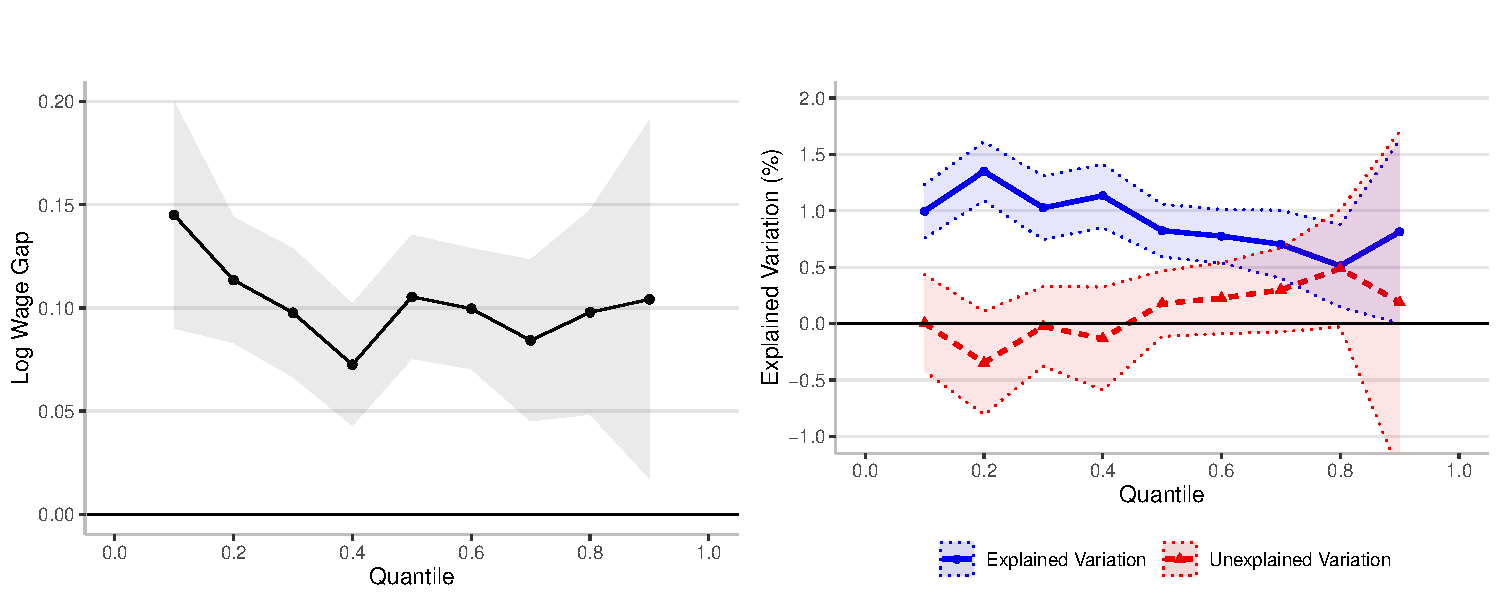
\includegraphics[scale=0.65]{nfgap}
			\caption{German Native-Foreign Wage Gap in the Baseline Sample, 1992-2018 \label{fig:wage_gap_base}}
		%	{\footnotesize NOTE. \textemdash The vertical difference between contributions from individual-level (``Indiv.'') variation in tasks and total variation (``Total'') reflects contributions from occupation-level variation in tasks. Therefore, the smaller this vertical gap, the more important is idiosyncratic variation relative to occupational variation .\par}
		%{\caption  {Contributions of Task Variation Within Occupations to the explained Native-Foreign Wage Gap with base task group Routine Manual, 1992-2018 \label{fig:wgap_within_baserm}}}
%width=1.\linewidth,
\end{figure}


\iffalse

\begin{figure}[htbp]
\centering
\begin{floatrow}
\ffigbox[\FBwidth]
{
\subfloat[Wage Gap: Distribution \label{fig:RIF_wgap}]{\includegraphics[scale=0.25]{RIF_4_wgap_all}} 
%RIF_5_wgap
\quad
\subfloat[Explained Wage Gap \label{fig:RIF_wgap_exp}]{\includegraphics[scale=0.25]{RIF_4_ind_occ_task_immi3}} 
}
{}
\captionsetup{justification=centering}
{\caption{German Native-Foreign Wage Gap in the Baseline Sample, 1992-2018 \label{fig:wage_gap_base}}}
\end{floatrow}
%\bigskip
%{\footnotesize NOTE. \textemdash All point estimates are supplemented by a 95\% Confidence Interval (CI) based on bootstrapped standard errors with 100 replications.\par}
\end{figure}

\fi
